In order to implement the application, first of all, a new project has to be created in Eclipse. This project is going to be a Papyrus project (figure \ref{fig:Papyrus Project}).

\begin{figure}
\centering
{\includegraphics[scale=0.3]{./chapter4/projPapyrus/Selection_001.png}}
\caption{New Papyrus Project}
\label{fig:Papyrus Project}
\end{figure}

The first field that has to be specified is the Architecture Context. Here, the default values are the right ones as an UML model is what is required to implement with Papyrus (figure \ref{fig:Architecture Context}).

\begin{figure}
\centering
{\includegraphics[scale=0.3]{./chapter4/projPapyrus/Selection_002.png}}
\caption{Architecture Context}
\label{fig:Architecture Context}
\end{figure}

After that, the name of the project has to be defined. Due to the fact that it is going to implement an application called Great Seller, the name of the Papyrus project is going to be greatSellerApp (figure \ref{fig:Project Name Definition}).

\begin{figure}
\centering
{\includegraphics[scale=0.3]{./chapter4/projPapyrus/Selection_003.png}}
\caption{Project Name Definition}
\label{fig:Project Name Definition}
\end{figure}

The next step is to select the representation kind and to choose the StreamGen profile. StreamGen requires Papyrus to make a class diagram representation and, as the StreamGen project is already in the Eclipse workspace, the profile can be found browsing in the workspace (streamgen/profile/StreamUML.profile.uml). As it can be seen in the figure \ref{fig:Representation Kind}.

\begin{figure}
\centering
{\includegraphics[scale=0.3]{./chapter4/projPapyrus/Selection_004.png}}
\caption{Representation Kind}
\label{fig:Representation Kind}
\end{figure}

Finally, we can finish with the new Papyrus project initialization (figure \ref{fig:Papyrus Project Definition}).

\begin{figure}
\centering
{\includegraphics[scale=0.3]{./chapter4/projPapyrus/Selection_005.png}}
\caption{Papyrus Project Definition}
\label{fig:Papyrus Project Definition}
\end{figure}

The next step is to define the model in the class diagram in order to specify that the application is going to be a Flink application. Then, first of all, we have to create a model node in the greatSellerApp.di file. This node is going to be called greatSeller as it is the object representing the whole application. Once the node is inserted, the properties of such node must be specified. More in detail, the Flink application stereotype has to be applied. In this case, the properties of the model has to be the default ones then nothing else must be done with the model node.

The next step is to add the data types that the application is going to need. In order to do this, a package node has to be inserted inside the Flink application model node. This package is called greatSellerDataTypes and a stereotype has to be applied as in the previous case. First of all, inside the properties window, in the profile field, the applied stereotype is defined. Inside this package all the datatypes that the application requires have to be inserted. The first data type is the InputTransactions which is composed of a transaction id (integer), a data subject (string), an amount (double) and a recipient id (string). The second data type is the IssuedTransactions which contains the data subject (string) and the number of transactions performed by such data subject which can be seen by means of the variable NTransactions (integer). The third data type is the SpentAmount which is composed of the data subject (string) and the total amount of money spent by the data subject which can be seen by means of the variable TotalAmount (double). Finally, the last data type is the NumberUsers which contains the number of users who spent more than 1000 dollars and it is represented by means of the variable NTopUsers (integer). Then, we need to insert one DataType node inside the package created in the previous step with each of these data types. Each data type can be seen as a tuple which is composed by several values. The name of the DataType node is going to be the same that the one corresponding to the tuple and each of the values that compose the tuple are going to be a property inside of the owned attributes that are specified in the UML field of the properties of each DataType node.

\begin{table}[h!]
\centering
	\begin{tabular}{||c|c|c||} 
	\hline\hline
	DataType & Properties & PropertyType \\ [1ex] 
	\hline\hline
	InputTransactions & transactionId & integer  \\
	& dataSubject & string  \\
	& amount & double  \\
	& recipientId & string  \\
	\hline
	IssuedTransactions & dataSubject & string  \\
	& nTransactions & integer \\
	\hline
	SpentAmount & dataSubject & string  \\
	& totalAmount & double \\
	\hline
	NumberUsers & NTopUsers & double  \\
	\hline\hline
	\end{tabular}
\caption{DataTypes Composition}
\label{DataTypes Composition}
\end{table}

\section{Files Generation}

\subsection{Source Files Generation}
In order to generate the text file that feeds the Great Seller DIA, two Python codes have been developed. In addition, a Map Transformation is implemented in the DIA in order to split the input strings generated by the Python codes and to generate the InputTransaction data type.

The first Python code builds a Python list which represents the Great Seller stock of 25 products and it assigns to each product a price. Each product is represented with a dictionary variable that contains a name variable and a price variable. The name variable is a string with the word 'product' immediately followed by an integer number from 1 to 25 which points to the product of the stock. The price is an integer number between \$1 and \$200 which is assigned randomly. Once the name and the price are assigned to the dictionary, the product is added to the stock list. Finally, the Great Seller stock list is saved in a binary shelf file in order to be accessible from the other Python code.

The second Python code generates the strings that represent the tuples produced by each consumer. In order to generate such tuples an integer number for the transactionId is assigned following an increasing numerical order from 1 to the maximum number of generated transactions which is input by command line to the code, it can be 10, 100 or 1000. After that, randomly, one of the four possible data subjects (Bob, Carlos, Elisabetta and Michele) and a product from the stock saved in the binary shelf file are assigned. Finally, each value is added to a string where each of these values are separated by a comma. The generated string represents the tuple produced by each consumer and it is written in the text file which is called from the Great Seller DIA in order to feed it.

Once, the DIA inputs each of this strings in a non-parallel stream, a Map Transformation, taking advantage of the split Java method, splits the strings by the comma generating the InputTransaction data type which is composed of four fields: transactionId, dataSubject, amount and product.


\subsection{Java Codes Generation}

In order to generate the Java codes from the Papyrus model, first of all we need to create a new Java project in Eclipse (File -$>$ New -$>$ Java Project). This project is going to be called 'greatSellerCodes' as it can be seen in the figure \ref{fig:Java Project Creation}.

\begin{figure}
\centering
{\includegraphics[scale=0.3]{./chapter4/javaCodesGeneration/Selection_001.png}}
\caption{Java Project Creation}
\label{fig:Java Project Creation}
\end{figure}

Once the Java project is created, its structure has to be modified in order to allow to be compatible with Maven. As the figure \ref{fig:Java Project Initial Structure} shows, firstly the Java project is composed of a JRE System Library and a src folder. This src folder has to be deleted, leaving the Java project only with the JRE System Library as it can be seen in the figure \ref{fig:Java Project Final Structure}.

\begin{figure}
\centering
{\includegraphics[scale=0.3]{./chapter4/javaCodesGeneration/Selection_002.png}}
\caption{Java Project Initial Structure}
\label{fig:Java Project Initial Structure}
\end{figure}

\begin{figure}
\centering
{\includegraphics[scale=0.3]{./chapter4/javaCodesGeneration/Selection_003.png}}
\caption{Java Project Final Structure}
\label{fig:Java Project Final Structure}
\end{figure}

The next step is to create a source folder with a predefined structure as it is going to be specified now. Firstly, in the properties for the project, in the Java Build Path field, a folder has to added as the figure \ref{fig:Maven Project Structure Creation} specifies. In the default output folder a specific structure has to be written, greatSellerCodes/src/main/java. After this is written, the changes have to be applied and then click on 'Add Folder...'.

\begin{figure}
\centering
{\includegraphics[scale=0.3]{./chapter4/javaCodesGeneration/Selection_004.png}}
\caption{Maven Project Structure Creation}
\label{fig:Maven Project Structure Creation}
\end{figure}

In order to create the source folder, the java folder has to be selected and then click on 'OK' as it is shown in figure \ref{fig:Maven Project Source Folder Creation}. Then the changes have to be applied and, then, the window Properties for greatSellerCodes has to be closed (figure \ref{fig:Maven Project Properties}).

\begin{figure}
\centering
{\includegraphics[scale=0.3]{./chapter4/javaCodesGeneration/Selection_005.png}}
\caption{Maven Project Source Folder Creation}
\label{fig:Maven Project Source Folder Creation}
\end{figure}

\begin{figure}
\centering
{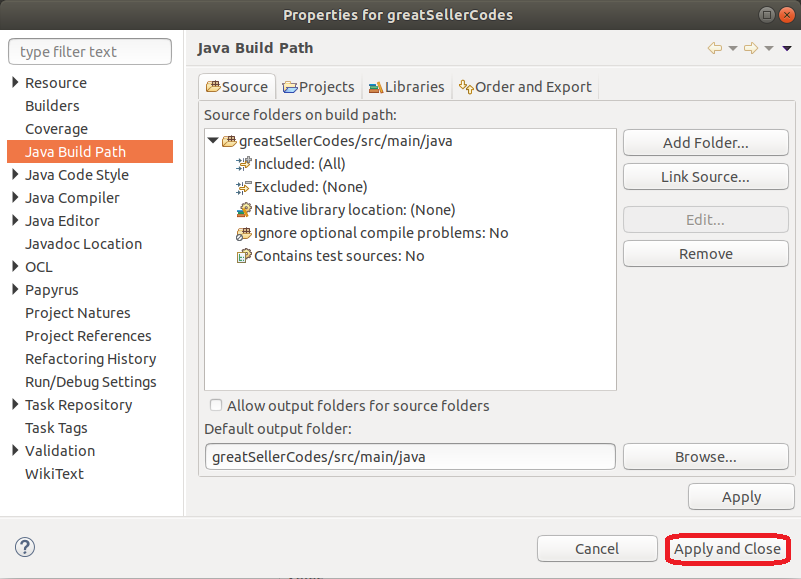
\includegraphics[scale=0.3]{./chapter4/javaCodesGeneration/Selection_006.png}}
\caption{Maven Project Properties}
\label{fig:Maven Project Properties}
\end{figure}

After these steps, the project folder should look like it is shown in the figure \ref{fig:Maven Project Structure} at the Package Explorer. And then, the project is ready to convert it into a Maven project. In order to do this, going to the 'Configure' option of the project and then clicking on 'Convert to Maven Project'. Then, a POM file has to be created and it is going to be created the default one as it can be seen in the figure \ref{fig:POM File Creation}. At this point, the structure of the project has to be the same that the one shown in the figure \ref{fig:Final Maven Project}.

\begin{figure}
\centering
{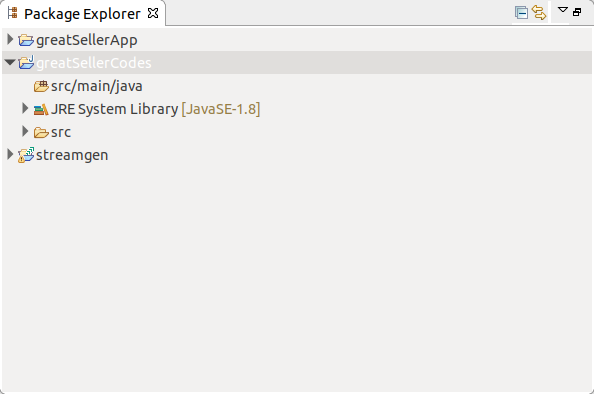
\includegraphics[scale=0.3]{./chapter4/javaCodesGeneration/Selection_007.png}}
\caption{Maven Project Structure}
\label{fig:Maven Project Structure}
\end{figure}

\begin{figure}
\centering
{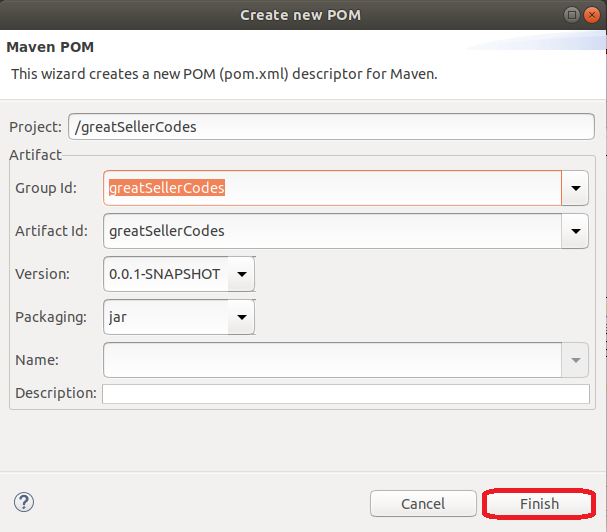
\includegraphics[scale=0.3]{./chapter4/javaCodesGeneration/Selection_008.png}}
\caption{POM File Creation}
\label{fig:POM File Creation}
\end{figure}

\begin{figure}
\centering
{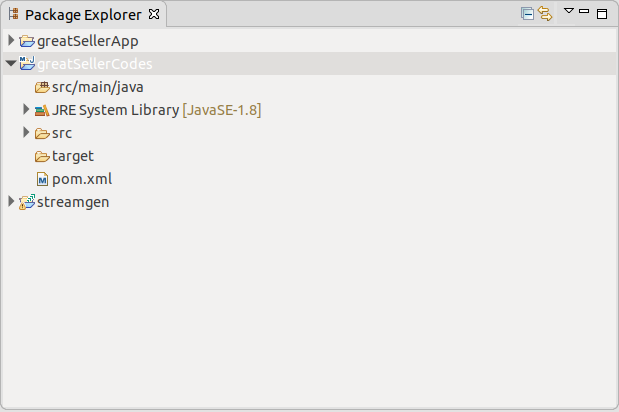
\includegraphics[scale=0.3]{./chapter4/javaCodesGeneration/Selection_009.png}}
\caption{Final Maven Project}
\label{fig:Final Maven Project}
\end{figure}

Now it is time to run the configuration (Run -$>$ Run Configurations...). In the figure \ref{fig:Run Configuration} is shown how this window has to be filled.

\begin{figure}
\centering
{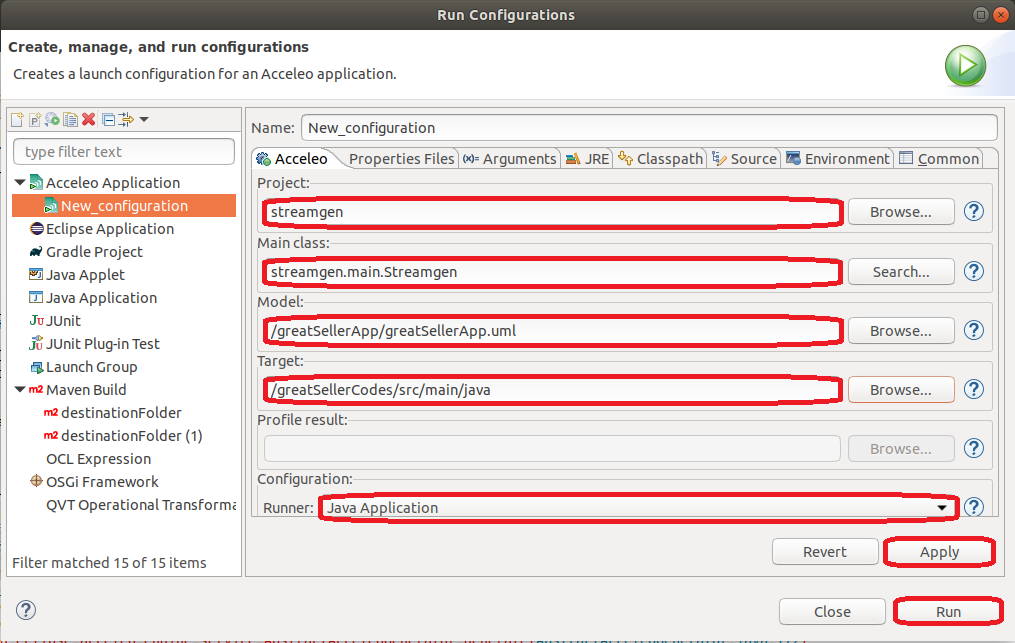
\includegraphics[scale=0.3]{./chapter4/javaCodesGeneration/Selection_010.png}}
\caption{Run Configuration}
\label{fig:Run Configuration}
\end{figure}

\section{Requirements}
The first requirements that are needed in order to develop the big data application is to install the corresponding versions of Eclipse, Papyrus and Acceleo. In spite of the application is able to work with other versions, some problems could appear because of the changes that they present. The models implemented in this document have been developed with the following versions:

\begin{itemize}
\item Eclipse 2019-03 (4.11.0).
\item Papyrus SysML 1.4 Feature	1.3.0.
\item Acceleo 3.7.8.201902261618.
\item m2e-Maven Integration for Eclipse (includes Incubating components) 1.11.0.20190220-2119.
\item Apache Flink 1.4.0.
\end{itemize}











